\chapter{Distributed Objects and Remove Invocation}
\begin{multicols*}{2}

\noindent Remote objects are objects that can receive remote invocations\\

\noindent Remote method invocation means method invocation between objects in different processes\\

\noindent Remote object reference is used to uniquely identify an object throughout a distributed system\\

\noindent Remote interface: each remote object has a remote interface specifying the methods that can be invoked remotely

\section{Invocation Semantics}

\scriptsize
\begin{center}
\begin{tabular}{ |m{2cm}|p{1.7cm}|p{1.7cm}|p{1.7cm}| } 
    \hline
    \multirow{2}{2cm}{\begin{center}Invocation Semantics\end{center}} & \multicolumn{3}{p{5.1cm}|}{Fault Tolerance Measures} \\ \cline{2-4}
    & Retransmit request message & Duplicate filtering & Re-execute method or retransmit reply \\
    \hline
    Maybe\newline  & No  & N/A & N/A \\
    \hline
    At-least-once  & Yes & No  & Re-execute method \\
    \hline
    At-most-once   & Yes & Yes & Retransmit reply \\
    \hline
\end{tabular}
\end{center}
\normalsize

\section{Architecture of RMI}

\begin{center}
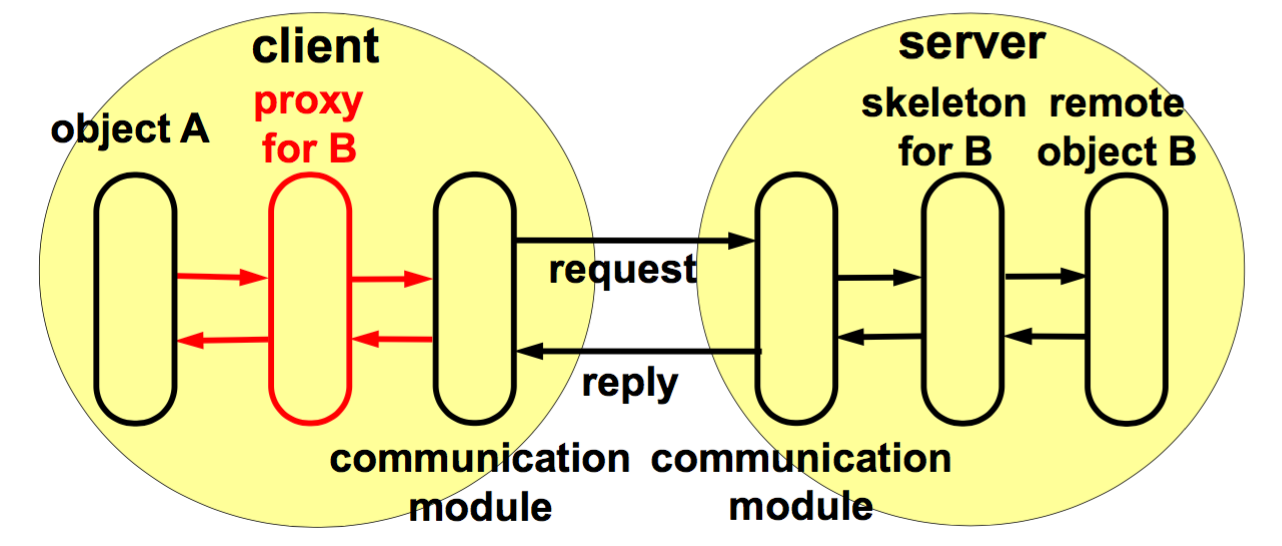
\includegraphics[width=8cm]{rmi-architecture}
\end{center}

\noindent One proxy for each class of remote objects. It marshals arguments and unmarshals results\\

\noindent Communication modules transmit request and reply message between client and server\\

\noindent One skeleton for each class of remote objects. It unmarshals arguments, invokes the corresponding method in the remote object, and marshals results\\

\noindent Binder is a name service that maintains mappings from object names to remote object references.

\section{Java RMI Architecture}

\noindent Step 1: Design the remote interface

\begin{minted}{Java}
public interface City extends Remote {
  int addInformation(String cityName, 
    String information)
    throws RemoteException;

  String getInformation(String cityName)
    throws RemoteException;
}
\end{minted}

\noindent Step 2: Design the servant class to implement the methods specified in the remote interface

\begin{minted}{Java}
public class CityImpl
    extends UnicastRemoteObject
    implements City {
  public CityImpl() throws RemoteException {
    super();
  }
  int addInformation(...) ...  { ... }
  String getInformation(...) ...  { ... }
}
\end{minted}

\noindent Step 3: Design the server class to create remote objects and register then in RMI registry

\begin{minted}{Java}
public class CityServer {
  public static void main(String args[]) {
    try {
      CityImpl aCityImpl = new CityImpl();
      Naming.rebind("rmi://.../City", 
          aCityImpl);
    } catch (Exception e) {...}
  }
}
\end{minted}

\noindent Step 4: Design the client  class to look up remote objects and access them

\begin{minted}{Java}
public class CityClient {
  public static void main(String args[]) {
    try {
      City aCityServer = 
          (City) Naming.lookup("rmi://.../City");
      aCityServer.getInformation(...);
    } 
    catch (RemoteException e) {...}
    catch (Exception e) {...}
  }
}
\end{minted}

\noindent Step 5: Compile remote interface, generating proxies, skeletons, and compile source codes\\

\noindent Step 6: Start server, followed by clients

\subsection{Implement Callback}

\noindent Callback: the server informs the client when the information is updated\\

\noindent Client create a remote object that implements “Remote” interface, which contains a method for server to call

\begin{minted}{Java}
public interface Callback extends Remote {
  void theMethod() throws RemoteException;
}

public class CityClient {
  public static void main(String args[]) {
    try {
      City aCityServer = 
          (City) Naming.lookup("rmi://.../City");
      Callback cb = new Callback();
      aCityServer.register(cb);
    } catch (RemoteException e) {
    }
  }
}
\end{minted}

\noindent Server provides “register” and “deregister” operation for interested clients. When an event of interest occurs, server invokes the method in callback objects

\begin{minted}{Java}
public interface City implements Remote {
  void register(Callback cbObject) 
      throws RemoteException;
  void deregister(Callback cbObject) 
      throws RemoteException;
}
\end{minted}

\end{multicols*}
